\usepackage{extarticle}
\documentclass[14pt]{extarticle}
\usepackage[paperheight=7in, paperwidth=10in, total={9.5in, 6.5in}]{geometry}
\usepackage{tikz}

\usetikzlibrary{automata, positioning, shapes.geometric, arrows.meta}

\tikzset{
    state/.style={
        ellipse, draw, fill={rgb:black,1;white,5},
        minimum size=10pt
    },
    box/.style={
        rectangle, draw, fill={rgb:black,1;white,5},
        minimum width=75pt, minimum height=50pt, align=center,
        anchor=north
    },
    mm/.style={
        -{Stealth[length=3mm]}
    },
    oo/.style={
        {Stealth[length=3mm]}-{Stealth[length=3mm]}
    },
    tikkup/.style={
        anchor=south west, rotate=20, align=left
    },
    tikkdown/.style={
        anchor=north east, rotate=20, align=right
    }
}

\begin{document}

\begin{center}
    {\Huge \bf Block Diagram of Autonomous Lawnmower} \\[45pt]
    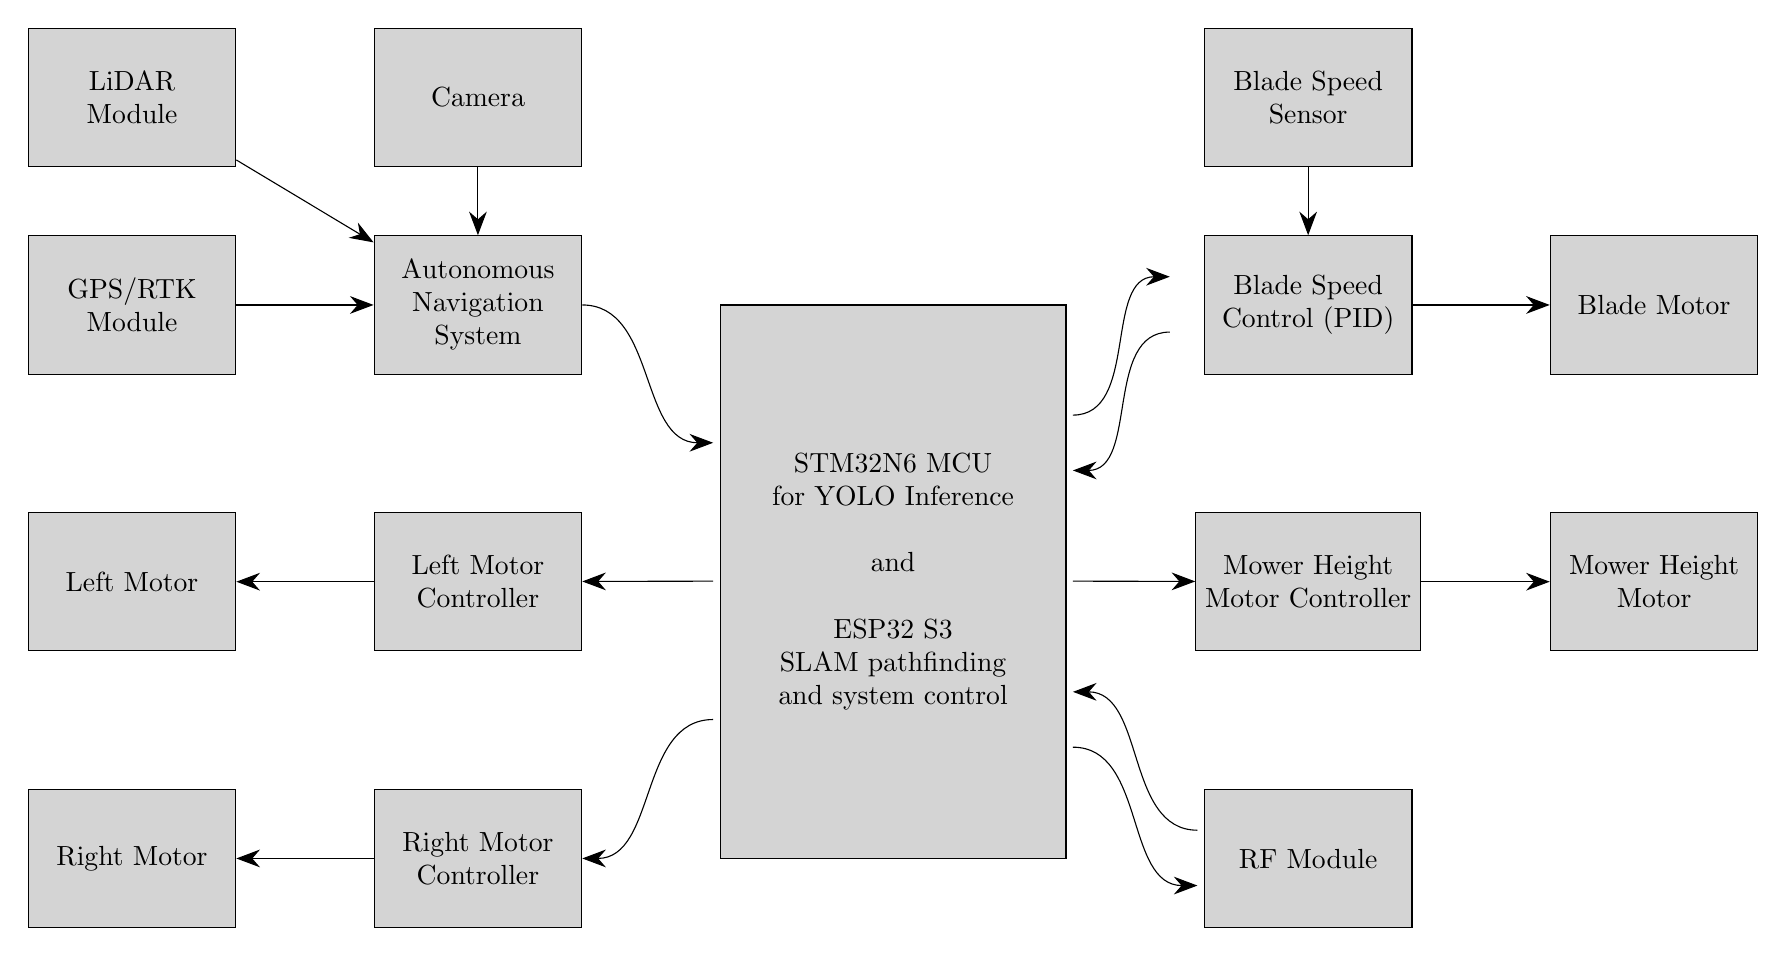
\begin{tikzpicture}[x=5pt, y=5pt]
        % \draw[help lines, step=5] (0,0) grid (130,90);
        % \node at (0,0) {O};
        
        \node[box, minimum height=200pt, minimum width=125pt]   (mcu)           at (65,60) {STM32N6 MCU\\for YOLO Inference\\\\and\\\\ESP32 S3\\SLAM pathfinding\\and system control};

        % Navigation system
        
        \node[box] (autonomous)    at (35,65) {Autonomous\\Navigation\\System};
        \node[box] (gps)           at (10,65) {GPS/RTK\\Module};
        \node[box] (lidar)         at (10,80) {LiDAR\\Module};
        \node[box] (computer)      at (35,80) {Camera};

        \path (autonomous) edge[mm, out=0, in=180] (52,50)
                (gps) edge[mm] (autonomous)
                (lidar) edge[mm] (autonomous)
                (computer) edge[mm] (autonomous);

        % Blade speed control

        \node[box] (speedcontrol)   at (95,65)  {Blade Speed\\Control (PID)};
        \node[box] (speedsensor)    at (95,80)  {Blade Speed\\Sensor};
        \node[box] (blademotor)     at (120,65) {Blade Motor};

        \path (85,58) edge[mm, out=180, in=0] (78,48)
                (78,52) edge[mm, out=0, in=180] (85,62)
                (speedcontrol) edge[mm] (blademotor)
                (speedsensor) edge[mm] (speedcontrol);

        % Mower height control

        \node[box] (heightcontroller)   at (95,45)  {Mower Height\\Motor Controller};
        \node[box] (heightmotor)        at (120,45) {Mower Height\\Motor};

        \path (78,40) edge[mm] (heightcontroller)
                (heightcontroller) edge[mm] (heightmotor);

        % RF Modules

        \node[box] (transmitter)    at (95,25)  {RF Module};

        \path (78,28) edge[mm, out=0, in=180] (87,18)
                (87,22) edge[mm, out=180, in=0] (78,32);

        % Motors and Motor Controllers

        \node[box] (leftcontrol)    at (35,45) {Left Motor\\Controller};
        \node[box] (leftmotor)      at (10,45) {Left Motor};
        \node[box] (rightcontrol)   at (35,25) {Right Motor\\Controller};
        \node[box] (rightmotor)     at (10,25) {Right Motor};

        \path (52,40) edge[mm] (leftcontrol)
                (leftcontrol) edge[mm] (leftmotor)
                (52,30) edge[mm, out=180, in=0] (rightcontrol)
                (rightcontrol) edge[mm] (rightmotor);
    \end{tikzpicture}
\end{center}
    
\end{document}